
\documentclass[licencjacka]{pracamgr}

\autor{Tomasz Kanas}{385674}

\title{Optymalna strategia podawania leku}

\tytulang{Optimal strategy of drug dosage}

\kierunek{matematyka}

\opiekun{dr. Piotr Krzyżanowski\\
  Instytut Matematyki Stosowanej i Mechaniki\\
}
\date{Wrzesień 2020}
\dziedzina{
  11.1 Matematyka\\
}
\klasyfikacja{49-XX Calculus of variations and optimal control; optimization\\
  49M37 Numerical methods based on nonlinear programming\\
  }

\keywords{teoria sterowania, programowanie nieliniowe, nowotwór, Octave}

\usepackage[utf8]{inputenc}
\usepackage{polski}
%\usepackage{romannum}
\usepackage{amsmath}
% \usepackage{amssymb}
\usepackage{amsfonts}
\usepackage{amsthm}
\usepackage{mathdots}
\usepackage{fullpage}
\usepackage{gensymb}
\usepackage{MnSymbol}
\usepackage{stmaryrd}
\usepackage{graphicx}
\usepackage{subcaption}
\usepackage{multirow}
\usepackage{dsfont}
\usepackage{url}

\def\R{\mathbb{R}}
\def\C{\mathbb{C}}
\def\Z{\mathbb{Z}}
\def\Q{\mathbb{Q}}
\def\N{\mathbb{N}}
\def\Rn{\mathbb{R}^n}
\def\E{\mathcal{E}}
\def\B{\mathcal{B}}
\def\1{\mathds{1}}
\def\nor{\trianglelefteq}
\def\ker{\operatorname{ker}}
\def\gengru#1{\langle\,#1 \,\rangle}
\def\ch{\blacktriangleleft}
\def\arr{\longrightarrow}
\def\Abs#1{\left\vert#1\right\vert}
\def\rk{\operatorname{rank}}
\def\lin{\operatorname{lin}}
\def\af{\operatorname{af}}
\def\dim{\operatorname{dim}}
\def\ker{\operatorname{ker}}
\def\im{\operatorname{im}}
\def\tr{\operatorname{tr}}
\def\Hom{\operatorname{Hom}}
\def\Aut{\operatorname{Aut}}
\def\id{\triangleleft}
\def\iif{\operatorname{if}}
\newcommand{\norm}[1]{\left\lVert#1\right\rVert}
\def\normsign{\|\cdot\|}
\newcommand{\series}[3]{\sum_{#1}^{#2}#3}

\newtheorem{problem}{Problem}
\newtheorem{definicja}{Definicja}
  
\begin{document}
\pagenumbering{arabic}
\maketitle

\begin{abstract}
  W pracy przedstawiono metodę numerycznego wyznaczania przybliżenia optymalnej strategii podawania leku przy leczeniu nowotworu.
  Sporządzono i opisano implementację metody w środowisku Octave oraz przeprowadzono i omówiono wyniki eksperymentów.
\end{abstract}

\tableofcontents

\chapter*{Wprowadzenie}
\addcontentsline{toc}{chapter}{Wprowadzenie}

Nowotwory są jednym z największych problemów współczesnej medycyny. Przyczyniają się one do bardzo wielu zgonów na całym świecie. Proces leczenia nowotworu nie zawsze jest skuteczny oraz potrafi być bardzo wyniszczający dla organizmu pacjenta, dlatego tak istotne jest, by terapia prowadzona była w jak najlepszy sposób.

W tej pracy przedstawimy metodę przybliżonego rozwiązania pewnego modelu przedstawiającego zależność między strategią podawania leku, a przebiegiem i skutecznością terapii. Celem naszym będzie znalezienie strategii podawania leku optymalizującą, podaną w tym modelu, miarę skuteczności terapii.

Do rozwiązania tego zadania sformułujemy je jako zadanie optymalizacji nieliniowej z ograniczeniami. Zaprojektujemy i zaimplementujemy algorytm poszukujący wspomnianej optymalnej strategii podawania leku. Przeprowadzimy też eksperymenty badające poprawność i skuteczność naszej implementacji, oraz wpływ jaki mają na nią rozmaite parametry wynikające z zastosowanej metody. Na końcu przeprowadzamy dyskusję uzyskanych wyników oraz użytych metod.

\chapter{Sformułowanie problemu}
Celem pracy jest znalezienie strategii podawania leku przy leczeniu nowotworu, pozwalającej osiągnąć możliwie największą skuteczność terapii. W tym celu skorzystamy z modelu przedstawionego w pracy \cite{BBF-manuscript} (zobacz też \cite{BBF2016}, \cite{BBF2019} gdzie przedstawiono podobne zagadnienia). Model ten przedstawia rozwój nowotworu w czasie w zależności od dawkowania leku, $g(t)$, za pomocą równania różniczkowego:
\begin{equation} \label{ode}
  \begin{aligned} 
    V_1'(t) &= \lambda_1V_1F\left(\frac{V_1 + \alpha_{12}V_2}{K}\right) - \beta_1V_1g(t), \\
    V_2'(t) &= \lambda_2V_2F\left(\frac{V_2 + \alpha_{21}V_1}{K}\right) - \beta_2V_2g(t), \\
    K'(t) &= -\mu K + (V_1+V_2) - d{(V_1 + V_2)}^{2/3}K - \beta K g(t) \\
  \end{aligned}
\end{equation}
dla $t \in [0, T]$, z warunkami początkowymi
\begin{equation} \label{ode-start}
   V_1(0) = V_{10},\ V_2(0) = V_{20},\ K(0) = K_0
\end{equation}
gdzie $F(x) = -\ln(x)$, $ 0 \le g(t) \le g_{\max}$, oraz
\[\lambda_1, \lambda_2, \alpha_{12}, \alpha_{21}, \beta_1, \beta_2, \beta, \mu, d, V_{10}, V_{20}, K_0 \]
są zadanymi nieujemnymi parametrami.

Funkcja $V_1(t)$ modeluje liczbę komórek guza podatnych na lek w momencie $t$, $V_2(t)$ liczbę komórek guza odpornych na lek, a $K(t)$ jest parametrem nazwanym w pracy ,,unaczynieniem''. Zauważmy, że rozwiązania $V_1, V_2, K$ zależą od wyboru funkcji $g$ którą nazywamy sterowaniem. W tym modelu wartość $g(t)$ ma interpretację jako wielkość dawki leku w czasie $t$.

Zgodnie z \cite{BBF-manuscript}, zadanie polega na znalezieniu funkcji $g: [0, T] \to [0, g_{\max}]$ takiej, że funkcje $V_1, V_2, K: [0, T] \to (0, \infty)$ spełniające (\ref{ode}) minimalizują funkcjonał:
\begin{equation} \label{objf}
  J(g, V_1, V_2, K) = \int_0^T V_1(t) + V_2(t)dt + \omega\int_0^T G\left(\frac{V_2(t) - V_1(t)}{\epsilon}\right) dt
\end{equation}
gdzie
\begin{equation*}
  G(x) = \frac{1+\tanh(x)}{2} \quad
  \omega, \epsilon > 0 
\end{equation*}

Problem ten w literaturze (np.~\cite{diehl},~\cite{rao-methods}) nazywa się problemem optymalnego sterowania.

\section{Problem wyjściowy}
Zdefiniujmy teraz formalnie problem oraz uprośćmy notację.

\begin{problem}\label{problem}
  Znaleźć funkcję kawałkami ciągłą
  \[g: [0, T] \to [0, g_{\max}],\]
  i funkcję
  \[y = {(y_1, y_2, y_3)}^T: [0,T] \to {(0, \infty)}^3,\]
  spełniającą równanie różniczkowe:
  \begin{equation}\label{odesim}
    \begin{aligned}
      \dot{y}(t) &= f(t, y, g), \\
      y(0) &= y_0 = {(y_{10}, y_{20}, y_{30})}^T,
    \end{aligned}
  \end{equation}
  minimalizujące funkcjonał
  \begin{equation}\label{objfsim}
    J(g, y) = \int_0^T y_1(t) + y_2(t)dt + \omega\int_0^T G\left(\frac{y_2(t) - y_1(t)}{\epsilon}\right) dt,
  \end{equation}
  gdzie $f = {(f_1, f_2, f_3)}^T$ jest określone wzorem
  \begin{equation}\label{dynamicsim}
    \begin{aligned}
      f_1(t, y, g) &= \lambda_1y_1F\left(\frac{y_1 + \alpha_{12}y_2}{y_3}\right) - \beta_1y_1g(t), \\
      f_2(t, y, g) &= \lambda_2y_2F\left(\frac{y_2 + \alpha_{21}y_1}{y_3}\right) - \beta_2y_2g(t), \\
      f_3(t, y, g) &= -\mu y_3 + (y_1+y_2) - d{(y_1 + y_2)}^{2/3}y_3 - \beta y_3 g(t). \\
    \end{aligned}
  \end{equation}
\end{problem}

Przez funkcję kawałkami ciągłą określoną na odcinku rozumiemy funkcję o skończonej liczbie punktów nieciągłości. Jako, że o funkcji $f$ zakładamy tylko kawałkami ciągłość, należy doprecyzować co rozumiemy przez (\ref{odesim}). Załóżmy, że punktami nieciągłości $f(t,y,g): \R^5 \to \R$ są $t = \xi_1,\ \ldots,\ \xi_n \in \R$, wtedy (\ref{odesim}) oznacza sekwencję równań różniczkowych postaci
\begin{equation}\label{nonconode}
  \begin{aligned}
    \dot{y}|_{(\xi_i, \xi_{i+1})}(t) &= f|_{(\xi_i, \xi_{i+1})}(t, y, g)\\
    y(\xi_i) &= \lim_{t\to \xi_i^-}y(t)
  \end{aligned}
  \quad \text{ gdzie } i \in \{0,\ldots, n\},\ \xi_0 = 0,\ \xi_{n+1}=T
\end{equation}

Zwróćmy jeszcze uwagę na fakt, że funkcja $F(x) = -\ln(x)$ posiada osobliwość w 0, więc prawa strona (\ref{dynamicsim}) nie jest dobrze zdefiniowana dla $y_1(t) = y_2(t) = 0$, a obliczenia w których argumenty $F$ są bliskie 0 mogą być obarczone dużymi błędami numerycznymi. Podobnie we wzorze (\ref{dynamicsim}) występuje dzielenie przez $y_3$, więc dla $y_3(t) = 0$ prawa strona (\ref{odesim}) także nie jest dobrze określona.

\section{Problem przybliżony}\label{simp_problem_subsec}
Wyznaczenie rozwiązania problemu optymalnego sterowania w postaci jawnego wzoru rzadko kiedy jest możliwe. Z tego powodu zdecydujemy się na szukanie rozwiązania przybliżonego.

Rozwiązanie Problemu~\ref{problem} przybliżymy rozwiązaniem pewnego problemu optymalizacji skończenie wymiarowej. W tym celu ustalimy siatkę dyskretyzacji przedziału $[0, T]$:
\begin{equation}
  0 = t_0 < t_1 < \cdots < t_{n-1} < t_n = T
\end{equation}
Możemy teraz przybliżać sterowanie $g$ za pomocą splajnu opartego na punktach $t_{i}$. Dla prostoty ograniczymy się do splajnów stopnia 0 i 1. Ostatecznie przybliżone sterowanie $\hat{g}$ ma postać:
\begin{gather}  
    \hat{g}(t) = g_i \text{ gdy } t \in [t_{i}, t_{i + 1}) \quad \text{(sterowanie kawałkami stałe)} \label{control_1}\\
    \nonumber \text{albo} \\
    \hat{g}(t) = \frac{(t_{i+1} - t)g_i + (t - t_i)g_{i+1}}{t_{i+1} - t_i} \text{ gdy } t \in [t_i, t_{i+1}) \quad \text{(sterowanie kawałkami liniowe)} \label{control_2}
\end{gather}
i jest jednoznacznie zdefiniowane przez wartości $g_i \simeq g(t_i)$ dla $i = 0,\ldots, n$. Te wartości będą optymalizowanymi zmiennymi.

Korzystając z przybliżonej funkcji sterowania, na każdym odcinku $[t_n, t_{n+1}]$ przybliżymy rozwiązanie $y$ równania różniczkowego (\ref{odesim}). Użyjemy do tego $M$ kroków metody Rungego-Kutty rzędu $r$ ze stałym krokiem długości $h = \frac{t_{n+1} - t_n}{M}$. Wtedy przybliżone rozwiązanie $\hat{y}(t) \simeq y(t)$ w punkcie $t = t_n + (m + 1)h$ dla $m = 0,\ldots, M$  wyraża się przez:
\begin{equation} \label{rk}
  \begin{split}
    &k_1 = f(t_n + mh, \hat{y}(t_n + mh), \hat{g}), \\
    &k_l = f(t_n + c_l h, \hat{y}(t_n + mh) + h \sum_{i = 1}^{l-1} a_{li}k_i, \hat{g}),\quad l = 2,\ldots, r \\
    &\hat{y}(t_n + (m+1)h) = \hat{y}(t_n + mh) + h \sum_{i = 1}^r b_i k_i,
  \end{split}
\end{equation}
gdzie $c_l, a_{li}, b_i$ są stałymi zależnymi od wybranej metody.

Zostało już tylko przybliżyć funkcjonał celu (\ref{objfsim}). Zapiszmy go w postaci
\begin{equation} \label{objf-sim}
  J(y) = \int_0^T j(y(t)) dt,
\end{equation}
gdzie
\begin{equation}
  j(y) = y_1 + y_2 + \omega G\left(\frac{y_2 - y_1}{\epsilon} \right).
\end{equation}
Wtedy ogólny wzór na kwadraturę ze stałym krokiem $h$ przybliżającą (\ref{objf-sim}) to
\begin{equation} \label{quad}
  Q(\hat{y}) = h\sum_{i = 0}^N \alpha_i j(\hat{y}(ih)),
\end{equation}
gdzie $N = \frac{T}{h}$, a $\alpha_i$ są stałymi zależnymi od wybranej kwadratury.

Zatem możemy zdefiniować przybliżoną funkcję celu jako funkcję $g_0,\ldots,g_n$:
\begin{equation}
  \hat{J}(g_0,\ldots, g_n) = Q(\hat{y}),
\end{equation}
ponieważ $\hat{y}$ jest jednoznacznie wyznaczony przez $\hat{g}$ za pomocą (\ref{rk}), a $\hat{g}$ jest wyznaczone jednoznacznie przez $g_0,\ldots,g_n$. Podsumowując, problem przybliżony to:
\begin{problem}\label{problemapprox}
  Znaleźć $g_0,\ldots, g_n$ minimalizujące
\begin{equation}\label{nlp}
  \hat{J}(g_0,\ldots, g_n),
\end{equation}
i spełniające
\begin{equation}\label{nlp_cons}
  \forall_{i \in \{0,\ldots,n\}} 0 \le g_i \le g_{\max}.
\end{equation}
\end{problem}

Jest to problem optymalizacji nieliniowej z ograniczeniami i istnieją implementacje metod pozwalających uzyskać przybliżone rozwiązanie tego problemu. To podejście do numerycznego problemu optymalnego nazywa się ,,direct single shooting'' i występuje np. w~\cite{diehl} i~\cite{rao-methods}.

\section{Alternatywne podejście}

Innym popularnym podejściem jest ,,direct collocation''. W tym podejściu zaczyna się, tak samo jak powyżej, od dyskretyzacji czasu:
\begin{equation}
  0 = t_0 < t_1 < \ldots < t_n = T.
\end{equation}
Następnie zarówno sterowanie jak i stan układu przybliża się splajnem opartym na punktach $t_i$. Dzięki temu sterowanie jest jednoznacznie wyznaczone przez wartości $g_i = \hat{g}(t_i)$, natomiast stan układu przez wartości $y_i = \hat{y}(t_i)$. Celem jest, tak samo jak powyżej, sprowadzenie problemu do problemu optymalizacji nieliniowej z ograniczeniami. Aby móc to zrobić należy znaleźć warunki jakie wartości $y_i$ muszą spełniać, aby układ spełniał w przybliżeniu równanie
\begin{equation}\label{ode-alternative}
  \dot{y}(t) = f(t,y(t),g(t)).
\end{equation}
Aby znaleźć te warunki przybliża się całkę z powyższego równania za pomocą pewnej kwadratury. Dla przykładu ustalmy kwadraturę trapezową. Wtedy dostajemy równanie przybliżone
\begin{equation}
  \int_{t_i}^{t_{i+1}} \dot{y}(t)dt = \int_{t_i}^{t_{i+1}} f(t,y(t),g(t))dt
\end{equation}
\begin{equation}
  y_{i+1} - y_{i} \simeq \frac{1}{2}(t_{i+1}-t_i)(f(t_{i+1}, y_{i+1}, g(t_{i+1})) - f(t_i, y_i, g(t_i))).
\end{equation}
Powyższy wzór dodaje się do ograniczeń optymalizatora jako ograniczenie równościowe. W ten sposób RRZ (\ref{ode-alternative}) zostaje w przybliżeniu wymuszone w rozwiązaniu.

Ograniczenia występujące w sformułowaniu oryginalnego problemu można zwykle bez problemu przekształcić na ograniczenia $g_i$ oraz $y_i$. Przybliżony funkcjonał celu definiuje się, jako numeryczne przybliżenie oryginalnego funkcjonału celu zastosowane do przybliżonego stanu $\hat{y}$ i sterowania $\hat{g}$.

Podejście to jest dokładnie opisane w~\cite{Kelly}, występuje też w~\cite{diehl} i~\cite{rao-methods}.

\section{Plan rozwiązania}
Aby obliczyć wynik problemu przybliżonego zdefiniowanego w rozdz.~\ref{simp_problem_subsec} zaimplementujemy przejście od problemu optymalnego sterowania do problemu optymalizacji nieliniowej z ograniczeniami. W tym celu skorzystamy ze środowiska MATLAB/Octave i dostarczonego w nim optymalizatora (FMINICON). Aby poprawić złożoność czasową optymalizacji i tym samym umożliwić stosowanie gęstszej siatki dyskretyzacji, obliczymy gradient przybliżonej funkcji celu. Będziemy też musieli znaleźć odpowiednią siatkę dyskretyzacji i punkt startowy dla optymalizatora. Należy też pamiętać, że dopuszczamy możliwość nieciągłości w sterowaniu, co może być przyczyną błędów przybliżenia i problemów ze zbieżnością optymalizacji. Zaimplementujemy rozwiązanie w taki sposób, aby ograniczyć problemy płynące z możliwej nieciągłości.

\chapter{Implementacja}
Optymalizator FMINICON wymaga dostarczenia funkcji do optymalizowania, czyli w naszym przypadku funkcji $\hat{J}$, oraz ograniczeń, czyli w przypadku metody ,,direct single shooting'' jedynie (\ref{nlp_cons}). Domyślnie optymalizator wyznacza gradient za pomocą różnic skończonych, co jest kosztowne, gdyż wymaga uruchomienia funkcji celu liniowo wiele razy względem liczby parametrów. Aby poprawić wydajność optymalizacji zaimplementujemy liczenie gradientu przybliżonej funkcji celu ze względu na parametry $g_0,\ldots, g_n$.

Zauważmy, że znalezienie dobrego wyniku będzie zapewne wymagało wielokrotnego wywołania naszej funkcji celu przez optymalizator, więc zależy nam aby funkcja celu liczyła się możliwie szybko. Lepsza wydajnościowo implementacja pozwoli też na większe zagęszczenie siatki dyskretyzacji i tym samym wzrost dokładności aproksymacji.

Jedną z praktyk pozwalającą poprawić wydajność programów w środowiskach MATLAB i Octave jest tak zwana wektoryzacja. Polega ona na zastępowaniu pętli operacjami na wektorach. Korzysta to z faktu, że wiele funkcji w tych środowiskach można wywołać z wektorem parametrów, zamiast pojedynczego parametru i zwracają one wtedy wektor wyników, oraz wykonują się znacznie szybciej niż gdyby wywołać je wielokrotnie w pętli, z pojedyńczymi argumentami. Z tego powodu będziemy korzystać z tej techniki gdzie to tylko możliwe.

Aby sprowadzić problem optymalnego sterowania do problemu optymalizacji nieliniowej musimy obliczyć przybliżone sterowanie (\ref{control_1}) lub (\ref{control_2}), przybliżyć rozwiązanie równania różniczkowego (\ref{rk}) a następnie za pomocą uzyskanego rozwiązania obliczyć kwadraturę (\ref{quad}) przybliżającą funkcję celu (\ref{objf}). Ponadto chcemy obliczyć gradient funkcji celu, co będzie wymagało policzenia pochodnej każdego z wymienionych wzorów względem parametrów $g_i$.

\section{Sterowanie}\label{subsec_sterowanie}
Jedynym problemem przy implementacji przybliżonego sterowania (\ref{control_1}) lub (\ref{control_2}) jest znalezienie indeksu $i$ takiego, że $t \in [t_{i-1}, t_i)$. Użyjemy do tego funkcji $lookup$, która wydajnie znajduje żądany indeks korzystając z wyszukiwania binarnego.

Aby policzyć gradient przybliżonego sterowania $\hat{g}$ ze względu na parametry $g_1,\ldots,g_n$ należy zróżniczkować równanie (\ref{control_1}) lub (\ref{control_2}):

\begin{gather}
  \frac{\partial \hat{g}}{\partial g_i}(t) = \begin{cases} 1 \text{ gdy } t \in [t_{i-1}, t_i) \\ 0 \text{ w.p.p.} \end{cases} \label{dcontrol_1}\\
  \nonumber \text{albo}\\
  \frac{\partial \hat{g}}{\partial g_i}(t) = \begin{cases} \frac{t_i - t}{t_i - t_{i-1}} \text{ gdy } t \in [t_{i-1}, t_i) \\ \frac{t - t_i}{t_{i+1} - t_i} \text{ gdy } t \in [t_{i}, t_{i+1}) \\ 0 \text{ w.p.p.} \end{cases} \label{dcontrol_2}
\end{gather}

Implementacja powyższych wzorów jest standardowa, znajdowanie odpowiedniego indeksu $i$ odbywa się tak samo, jak przy liczeniu wartości przybliżonego sterowania.

Zarówno funkcja $lookup$ jak i pozostałe operacje wykorzystywane do policzenia przybliżonego sterowania i jego gradientu są zwektoryzowane. W szczególności, środowiska MATLAB i Octave umożliwiają wektorowe indeksowanie, więc nasza implementacja sterowania i jego gradientu też jest zwektoryzowana.

\section{Równanie różniczkowe}\label{subsec_rrz}
Aby przybliżyć rozwiązanie równania (\ref{ode}) należy zaimplementować funkcję $f(t,y,g)$, a następnie bezpośrednio zaimplementować odpowiednią metodę Rungego-Kutty (\ref{rk}). Wzory te implementuje się bezpośrednio.

Liczenie pochodnych $\frac{\partial \hat{y}}{\partial g_i}$ polega na zróżniczkowaniu wzorów (\ref{rk}):
\begin{gather}
    \frac{\partial k_1}{\partial g_i} = D_f \cdot \frac{\partial \hat{y}}{\partial g_i}(t_n + mh) + \frac{\partial f}{\partial g_i}(t_n + mh, \hat{y}(t_n + mh), \hat{g}) \nonumber \\
    \frac{\partial k_l}{\partial g_i}  = D_f \cdot \left(\frac{\partial \hat{y}}{\partial g_i}(t_n + mh) + h\sum_{j=1}^{l-1} a_{lj}\frac{\partial k_i}{\partial g_j} \right) + \frac{\partial f}{\partial g_i}(t_n + mh, \hat{y}(t_n + mh), \hat{g})  \label{drk}\\
    \frac{\partial \hat{y}}{\partial g_i}(t_n + (m+1)h) = \frac{\partial \hat{y}}{\partial g_i}(t_n + mh) + h\sum_{j=1}^r b_j \frac{\partial k_j}{\partial g_i} \nonumber
\end{gather}
gdzie
\begin{equation} \label{Df}
  D_f = {\left[\frac{\partial f_i}{\partial y_j}\right]}_{i,j = 1,\ldots, 3} (t_n + ah, \hat{y}(t_n + mh), \hat{g})
\end{equation}
Wzory na elementy macierzy $D_f$ pominiemy, liczy się je i implementuje standardowo.

Nasza implementacja umożliwia też przekazanie wektora punktów w czasie jako argumentu. W takim przypadku wyliczane wartości w podanych punktach będą spamiętywane w trakcie optymalizacji i zwrócone w wyniku. Dla wygody założymy, że punkty podane będą w kolejności rosnącej, oraz odległości między sąsiednimi punktami będą podzielne przez długość kroku $h$. Dzięki temu założeniu potencjalne punkty nieciągłości naszego przybliżonego sterowania będą zawsze wypadały między krokami metody R-K, dzięki czemu pojedynczy krok algorytmu będzie przybliżał rozwiązanie równania różniczkowego o ciągłej prawej stronie, co jest jednym z założeń metody R-K.

\section{Funkcja celu}
Przybliżoną funkcję celu (\ref{quad}) można zaimplementować za pomocą iloczynu skalarnego:
\begin{equation}
  Q(\hat{y}) = {\left(h(\alpha_0),\ldots,h(\alpha_N)\right)}^T \cdot {j(\hat{y}(0, h, 2h, \ldots, T))}
\end{equation}

Zauważmy, że korzystamy tu, dla prostoty, z tej samej długości kroku, co w (\ref{rk}).

W implementacji w Octave korzystamy ze zwektoryzowanej implementacji funkcji $\hat{y}$. Implementacja funkcji $j$ też jest zwektoryzowana, ponieważ środowisko dostarcza nam zwektoryzowaną funkcję $\tanh$, a pozostałe operacje wektoryzują się naturalnie.

Gradient funkcji celu możemy zaimplementować jako mnożenie wektora przez macierz:
\begin{equation}
  {\left[\frac{\partial J}{\partial g_i}\right]}_{i = 0, \ldots n} = {\left(h(\alpha_0),\ldots,h(\alpha_N)\right)}^T \cdot {\left[\frac{\partial j(\hat{y}(hi))}{\partial g_k}\right]}_{i = 0, \ldots N, k = 1, \ldots n}
\end{equation}
gdzie
\begin{equation}
  \frac{\partial j(y(t))}{\partial g_i} = \frac{\partial y_1(t)}{\partial g_i} + \frac{\partial y_2(t)}{\partial g_i} + \omega G'\left(\frac{y_2(t) - y_1(t)}{\epsilon}\right)\frac{\frac{\partial y_2(t)}{\partial g_i} - \frac{\partial y_1(t)}{\partial g_i}}{\epsilon},\quad G'(x) = \frac{1}{2\cosh^2(x)}
\end{equation}
\chapter{Eksperymenty}
W eksperymentach, do przybliżania rozwiązania równania (\ref{odesim}), będziemy korzystać z metody Rungego-Kutty 4-tego rzędu, ponieważ daje ona dobrą dokładność, a liczenie wartości funkcji $f$ nie jest zbyt kosztowne. Wartości stałych $c_l$, $a_{li}$, $b_i$ z wzoru (\ref{rk}) podane na tabeli Butchera:
\begin{equation}\label{butcher}
  \begin{array}
    {c|cccc}
    0\\
    \frac{1}{2} & \frac{1}{2}\\
    \frac{1}{2} &0 &\frac{1}{2} \\
    1& 0& 0& 1\\
    \hline{}
    & \frac{1}{6} &\frac{1}{3} &\frac{1}{3} &\frac{1}{6} 
  \end{array}
\end{equation}
Do przybliżania funkcjonału celu (\ref{objf}) użyjemy kwadratury trapezów. Kwadratura (\ref{quad}) wyraża się więc przez:
\begin{equation} \label{trapezoidal}
  Q(\hat{y}) = h\left(\frac{1}{2}(j(\hat{y}(0)) + j(\hat{y}(T))) + \sum_{i=1}^{N-1} j(\hat{y}(ih))\right)
\end{equation}

\section{Zbiór testowy}
Opiszemy teraz szeroki zbiór testowy, dobrany w taki sposób, aby móc zbadać wpływ różnych czynników na ostateczny wynik optymalizacji.
\subsection{Zestawy parametrów}
Użyjemy wartości parametrów podanych w wyjściowej pracy~\cite{BBF-manuscript}:
\begin{align*}
  t_0 &= 0          & \lambda_1 &= 0.192 & g_{\max} &= 3    \\
  T &= 200          & \lambda_2 &= 0.192 & \epsilon &= 0.01 \\
  V_{10} &= 20      & \beta_1 &= 0.15    & d &= 0.00873     \\
  V_{20} &= 280     & \beta_2 &= 0.1     & \mu &= 0         \\
  K_0 &= 650        & \beta &= 0.05      &       &          \\
\end{align*}
Wartości parametrów $\alpha_{12},\ \alpha_{21},\ \omega$ nie zostały ustalone w pracy, jedyne co jest ustalone to
\[ \alpha_{12} < \alpha_{21}\quad 0 < \omega \le 2000 \]
więc zbadamy problem dla 2 arbitralnie wybranych zestawów wartości tych parametrów (oznaczamy jako ,,Param.'' w tabelach z wynikami):
\begin{itemize}
\item{(CC)} $\quad \alpha_{12} = 0.1 \quad \alpha_{21} = 0.15 \quad \omega = 1000$
\item{(DC)} $\quad \alpha_{12} = 0.5 \quad \alpha_{21} = 0.75 \quad \omega = 2000$ 
\end{itemize}
\subsection{Algorytmy}
Do eksperymentów użyte zostało środowisko Octave. Funkcja FMINICON dostępna w pakiecie Optim~\cite{optim} umożliwia użycie jednego z dwóch algorytmów do optymalizacji nieliniowej:
\begin{itemize}
\item{\it lm\_feasible\/} oznaczany w tabelach {\it lm\/}

  Algorytm ten opiera się na algorytmie Levenberga–Marquardta, zob.~\cite{Kelley}. Implementacja tego algorytmu w Octave gwarantuje spełnianie ograniczeń w każdym kroku optymalizacji.
  
\item{\it sqp\/}
  
  Algorytm ten jest implementacją algorytmu sekwencyjnego programowania kwadratowego (ang. Sequential Quadratic Programming), zob.~\cite{Boggs}. Implementacja tego algorytmu w Octave gwarantuje spełnienie ograniczeń jedynie na końcu procesu optymalizacji.  
\end{itemize}

\subsection{Metody dyskretyzacji}
Do dyskretyzacji sterowania użyjemy dwóch metod (oznaczane ,,aproks.'' tabelach z wynikami):
\begin{itemize}
\item{$P_0$:} wykorzystująca splajny kawałkami stałe, zob. (\ref{dcontrol_1})
\item{$P_1$:} wykorzystująca splajny kawałkami liniowe, zob. (\ref{dcontrol_2})
\end{itemize}
Splajny te opierają się na siatce która, na użytek eksperymentu, może być jednego z trzech rodzajów (oznaczane ,,siatka'' w tabelach z wynikami):
\begin{itemize}
\item{$S_{\tau}$:} jednorodna, z krokiem $\tau$, więc $t_n = \tau n$. Ograniczymy się do $\tau \in \{0.1, 0.5, 1, 4\}$.
\item{$N_{sr}$: Niejednorodna, gęstsza w środku,} $t_n = \begin{cases}
    n \quad \text{gdy } n \le 25 \\
    25 + 0.1\cdot(n-25) \quad \text{gdy } 25 < n \le 525 \\
    75 + (n - 525) \quad \text{gdy } n > 525
  \end{cases}$
\item{$N_{kon}$: Niejednorodna, gęstsza na końcach,} $t_n = \begin{cases}
    0.5\cdot n \quad \text{gdy } n \le 100 \\
    50 + (n - 100) \quad \text{gdy } 100 < n \le 200 \\
    150 + 0.5\cdot (n - 200) \quad \text{gdy } n > 200
  \end{cases}$
\end{itemize}
\subsection{Krok dyskretyzacji $h$ metody R-K rozwiązania (\ref{odesim})}
Ograniczymy się do $h \in \{0.02, 0.1, 0.5\}$.
\subsection{Sterowania startowe}\label{start_control}
Optymalizator FMINICON wymaga podania początkowego przybliżenia sterowania optymalnego. Rozpoczęcie optymalizacji od odpowiednio dobrego sterowania może być niezbędne do uzyskania dobrych wyników, choć istnieją metody optymalizacji pozwalające osiągać dobre rezultaty nawet przy niezbyt dobrym przybliżeniu początkowym. Jest to bardzo przydatne w zadaniach w których nie znamy dobrego punktu startowego. Czasem jednak wiedza ekspercka pozwala ustalić dobre przybliżenie początkowe które wystarczy lekko poprawić aby uzyskać optimum. W naszym przypadku nie znamy dobrych kandydatów na sterowanie startowe. Przetestujemy więc sterowania ekstremalne (stale równe 0 lub $g_{\max}$) oraz sterowania kawałkami stałe postaci
\begin{equation}\label{start-parametrization}
  g_{\alpha,\beta,\gamma} = \alpha \cdot \1_{[t_0, \gamma)} + \beta \cdot \1_{[\gamma, T)}.
\end{equation}
Ograniczymy się do: $g_{0,0.55,42.5},\ g_{0.07,0.59,48.2}$. Zastosowane sterowanie startowe będzie podane w kolumnie ,,start'' w tabelach z wynikami.

\subsection{Heurystyczna metoda znajdowania sterowania startowego}\label{start_method}

Aby znaleźć sterowanie startowe które pozwoli uzyskać dobre wyniki, posłużyliśmy się pewną heurystyczną metodą. Będziemy szukać punktu startowego kawałkami stałego z maksymalnie jednym punktem nieciągłości.  Zauważmy, że sterowanie takie można sparametryzować trzema wartościami, co zrobiono w (\ref{start-parametrization}). Aby uzyskać jak najlepszy punkt startowy tej postaci, dostosowaliśmy naszą implementację rozwiązania problemu do podanej parametryzacji, czyli optymalizowaliśmy problem
\begin{equation}
  \min_{\alpha,\beta,\gamma} \check{J}(\alpha,\beta,\gamma) := \hat{J}(\alpha, \beta)\quad \text{z dyskretyzacją } t = (t_0, \gamma, T)
\end{equation}
i z ograniczeniami
\begin{equation}
  0 \le \alpha,\beta \le g_{\max}, \quad t_0 < \gamma < T.
\end{equation}
Zauważmy, że ta metoda jest heurystyczna, ponieważ nie wiemy czy $\check{J}(\alpha,\beta,\gamma)$ zależy od $\gamma$ w sposób różniczkowalny, ani nawet ciągły. Z tego też powodu nie mogliśmy policzyć analitycznie gradientu dla tego zadania i skorzystaliśmy z metody różnic skończonych. Aby otrzymać dobre rezultaty trzeba było uważnie ustawić parametr zatrzymania optymalizacji (,,TolFun''), oraz długość kroku różnic skończonych. Warto jeszcze nadmienić, że przez takie sformułowanie problemu nie mamy gwarancji, że punkt nieciągłości wypada między krokami algorytmów R-K (\ref{rk}) i kwadratury (\ref{quad}), co może skutkować znacznym błędem w wynikach tych metod na jednym przedziale długości $h$. Z tego powodu zastosowano wartość $h = 0.05$, niższą niż w większości eksperymentów.

Pomimo heurystyczności tej metody, udało się za jej pomocą uzyskać sterowanie $g_{0.07,0.59,48.2}$, które osiągnęło najlepsze wyniki w eksperymentach.

\subsection{Warunek stopu}
Algorytm {\it lm\/} kończy optymalizację gdy spełniony jest jeden z kilku warunków. Jednym z nich jest zbyt niewielka względna poprawa funkcji celu. Minimalna wartość tej poprawy jest ustawiana w FMINCON parametrem ,,TolFun''. Domyślną wartością tego parametru jest $10^{-4}$.

Podobnie dla algorytmu {\it sqp\/} istnieje w Octave parametr ,,octave\_sqp\_tolerance'', który odpowiada za różne kryteria stopu (niestety dokumentacja nie precyzuje za które). Domyślną wartością tego parametru jest pierwiastek z precyzji arytmetyki, czyli ok. $10^{-8}$.

W eksperymentach przetestujemy wpływ obu tych parametrów na proces optymalizacji. Dla prostoty oznaczmy oba te parametry przez ,,Tol'', co oznacza, że gdy testujemy algorytm {\it lm\/} to przez ,,Tol'' mamy na myśli ,,TolFun'', a gdy testujemy {\it sqp}, to mamy na myśli ,,octave\_sqp\_tolerance''. Przetestujemy wartości $\text{Tol} \in \{10^{-6}, 10^{-9}, 10^{-11}, 10^{-13}\}$. 

\section{Wyniki eksperymentów}
Jako, że powyższy zbiór jest duży, wykorzystamy jedynie niektóre testy. Przeprowadzimy kilka eksperymentów, każdy eksperyment będzie przeprowadzony na podzbiorze zbioru testowego, wybranym tak, aby zaprezentować wpływ konkretnego parametru na wyniki.

Wyniki eksperymentów będziemy oceniać na podstawie kilku wartości: wartości przybliżonego funkcjonału celu $\hat{J}$, liczby iteracji optymalizatora (oznaczaną przez ,,iter''), oraz liczbę wywołań funkcjonału celu w trakcie optymalizacji (oznaczaną przez $\#\hat{J}$).

Podamy też wartości pomagające ocenić jak blisko jest rozwiązaniu do faktycznego minimum lokalnego. W zadaniach optymalizacji z ograniczeniami częstym warunkiem stopu optymalizatora jest zerowanie się gradientu Lagrangianu wynikającego z warunków KKT.\ Jest to opisane np.\ w~\cite{diehl}. W naszym przypadku ograniczenia (\ref{nlp_cons}) mają prostą postać, więc gradient wspomnianego Lagrangianu upraszcza się do
\begin{equation}\label{lagrangian}
  \nabla L = {(l_i)}^T_{i = 0,\ldots, n} \quad \text{gdzie} \quad
  l_i = \begin{cases}
    0\ \quad \text{gdy } g_i = 0 \land \frac{\partial \hat{J}}{\partial g_i} > 0 \\
    0\ \quad \text{gdy } g_i = g_{\max} \land \frac{\partial \hat{J}}{\partial g_i} < 0 \\
    \frac{\partial \hat{J}}{\partial g_i}\ \text{w.p.p.}
  \end{cases}
  .
\end{equation}
Będziemy podawać normę gradientu Lagrangianu dla punktu zakończenia optymalizacji $\norm{L}_1$, oraz normę względną, czyli stosunek normy gradientów w punkcie zakończenia optymalizacji i w punkcie startowym: $\frac{\norm{L}_1}{\norm{L_0}_1}$.

Wartości funkcji celu są duże, więc dla zwiększenia czytelności będziemy podawać wartości dla $10^{-5}\hat{J}$ zaokrąglone do 2 miejsc po przecinku. Podobnie, dla normy lagrangianu będziemy podawać wartość $10^{-5}\norm{L}_1$ zaokrągloną do 2 miejsc po przecinku. Wartość normy względnej $\frac{\norm{L}_1}{\norm{L_0}_1}$ będziemy podawać zaokrągloną do 3 miejsc po przecinku, lub (gdy jest mniejsza niż $10^{-2}$) w postaci wykładniczej z dwoma cyframi znaczącymi.

\subsection{Test poprawności liczenia gradientu}
Pierwszy eksperyment ma na celu zaprezentowanie poprawności implementacji obliczania gradientu funkcji celu. Aby to sprawdzić porównamy naszą implementację, z domyślną implementacją przybliżającą gradient za pomocą różnic skończonych (FD) dostępną w FMINICON.\ Obliczanie wyników metodą domyślną wymaga wiele czasu, więc eksperyment obejmie tylko jeden przypadek, opisany na Tabeli~\ref{test_tbl}. Celem tego eksperymentu jest sprawdzenie poprawności implementacji, więc ograniczymy liczbę iteracji optymalizatora do 20, oraz pominiemy podawanie norm gradientów.
\begin{table}[h]
  \begin{center}
    \begin{tabular}{|p{1.7cm}|c|c|c|c|c|c|c|c|c|}
      \hline
      Gradient & Parametry & algorytm & aproks. & siatka & $h$ & start & $\hat{J}$ & iter & $\#\hat{J}$ \\
      \hline
      FD & (CC) & {\it lm\/} & $P_0$ & $S_4$ & 0.1 & $g_0$ & $3.26$ & 20 & 38 \\
      \hline
      wg. rozdz. \ref{subsec_sterowanie}, \ref{subsec_rrz} & (CC) & {\it lm\/} & $P_0$ & $S_4$ & 0.1 & $g_0$ & $3.25$ & 20 & 37 \\
      \hline
    \end{tabular}
    \caption{Test implementacji gradientu}\label{test_tbl}
  \end{center}
\end{table}

\begin{figure}[h]
  \begin{subfigure}{.5\textwidth}
    \caption{Rozwiązanie przy użyciu różnic skończonych}\label{nograd_sol}
    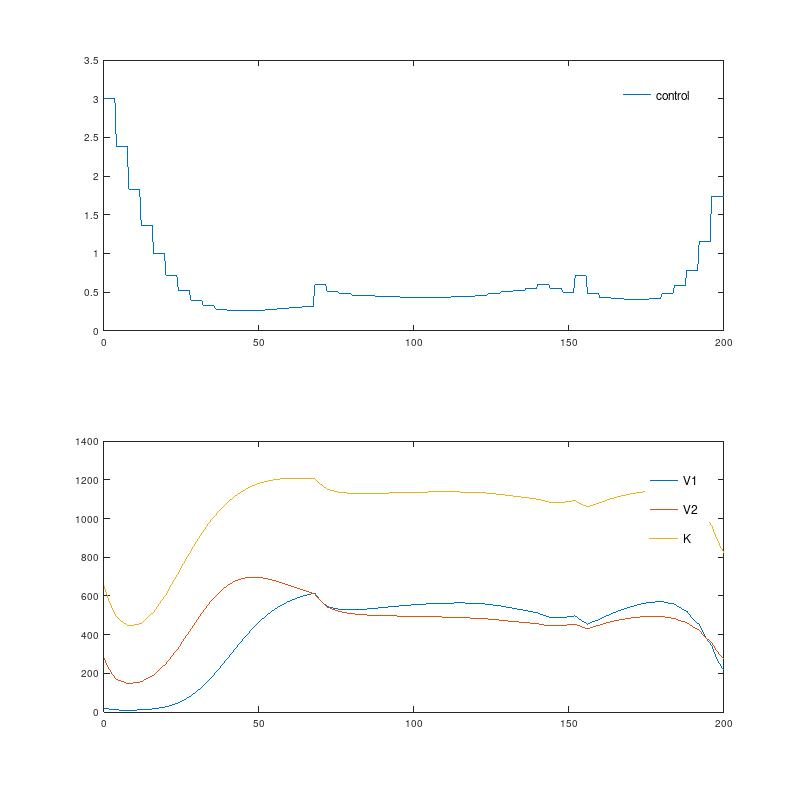
\includegraphics[width=\textwidth]{../plots/plot_nograd}
  \end{subfigure}
  \begin{subfigure}{.5\textwidth}
    \caption{Rozwiązanie z liczeniem gradientu}\label{test_sol}
    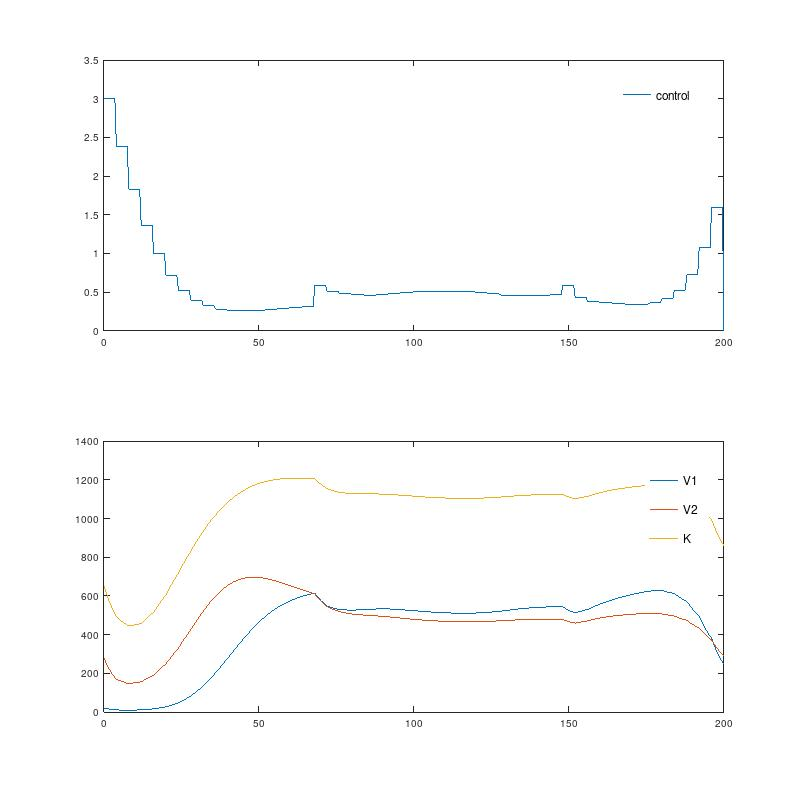
\includegraphics[width=\textwidth]{../plots/plot_test}
  \end{subfigure}%
  \caption{Rozwiązania dla przypadku testowego}\label{test_nograd_sol}
\end{figure}
Rozwiązania uzyskane obiema metodami są bardzo podobne, o czym świadczą wyniki zaprezentowane na Tabeli~\ref{test_tbl} i Rysunku~\ref{test_nograd_sol}. Ponadto nasza implementacja osiągnęła minimalnie lepszy wynik.

Dodatkowo policzymy gradient $G$ w punkcie będącym sterowaniem zaprezentowanym na wykresie~(\ref{test_sol}), oraz obliczymy przybliżenie $G_\tau$ tego gradientu za pomocą metody FD z krokiem $\tau$, dla różnych wartości kroku:
\[\tau \in \{10^{-3},10^{-4},\ldots,10^{-10}\}.\]
Następnie dla każdego $\tau$ obliczymy normę różnicy: $\norm{G - G_\tau}_1$. Wyniki tych obliczeń przedstawiamy na Tabeli~\ref{grad_fd_tbl}.

\begin{table}[h!]
  \begin{center}
    \begin{tabular}{|c|c|c|c|c|c|c|c|c|}
      \hline
      $\tau$ & $10^{-3}$ & $10^{-4}$ & $10^{-5}$ & $10^{-6}$ & $10^{-7}$ & $10^{-8}$ & $10^{-9}$ & $10^{-10}$ \\
      \hline
      $\norm{G - G_\tau}_1$ & 444599.7 & 34471.1 & 357.2 & 3.6 & 0.5 & 4.7 & 54.0 & 384.5 \\
      \hline
    \end{tabular}
    \caption{Różnice wyników między naszą implementacją gradientu, a różnicami skończonymi.}\label{grad_fd_tbl}
  \end{center}
\end{table}

Zgodnie z oczekiwaniami, gdy krok różnic skończonych $\tau$ maleje, to do pewnego momentu maleje też $\norm{G - G_\tau}_1$. W pewnym momencie norma ta zaczyna rosnąć wraz z dalszym zmniejszaniem $\tau$, gdyż dla tak niskich wartości $\tau$ obliczanie różnic dzielonych obarczone jest znacznym błędem numerycznym.

Warto tu jeszcze dodać, że liczba wywołań $\hat{J}$ podana w Tabeli~\ref{test_tbl} nie uwzględnia wywołań potrzebnych do aproksymacji gradientu metodą różnic skończonych. Aby policzyć pochodną dla jednego parametru potrzeba raz dodatkowo wywołać $\hat{J}$, więc jednorazowe policzenie gradientu wymaga tylu wywołań ile jest parametrów (w tym przypadku 51). Gradient jest liczony w każdej iteracji, co daje łącznie $20\cdot 51 = 1020$ dodatkowych wywołań $\hat{J}$. Inną wadą przybliżania gradientu metodą różnic skończonych są błędy. Zauważmy, że w okolicy punktu przecięcia się krzywych $y_1$ i $y_2$, wartość i pochodna wyrażenia $G((y_2(t) - y_1(t))/\epsilon)$, gdzie $G(x) = \frac{1 + \tanh(x)}{2}$, zmienia się bardzo szybko w czasie, co powoduje znaczne błędy przy zbyt dużym kroku metody różnic skończonych. Możemy je zaobserwować na Tabeli~\ref{grad_fd_tbl}, w postaci dużej normy różnicy gradientów, gdy krok różnic skończonych to $10^{-3}$. Wartość $10^{-3}$ jest wartością domyślna w FMINICON i została użyta do obliczenia wyników tego eksperymentu. Oznacza to w szczególności, że powyższe wyniki uzyskane przy użyciu FD są zapewne bardzo odległe od optymalnych.

\subsection{Parametry (CC)}

\begin{table}[h]
  \begin{center}
    \begin{tabular}{|c|c|c|c|c|c|c||c|c|c|c|c|}
      \hline
      Param. & algorytm & aproks. & siatka & $h$ & start & Tol & $\hat{J}$ & iter & $\#\hat{J}$ & $\norm{L}_1$ & $\frac{\norm{L}_1}{\norm{L_0}_1}$ \\
      \hline
      (CC) & {\it lm\/} & $P_0$ & $S_1$ & 0.1 & $g_0$ & $10^{-6}$ & 2.2 & 3 & 8 & 0.32 & 0.059 \\
      \hline
      (CC) & {\it lm\/} & $P_0$ & $S_1$ & 0.1 & $g_0$ & $10^{-9}$ & 2.2 & 64 & 69 & 0.32 & 0.059 \\
      \hline
      (CC) & {\it lm\/} & $P_0$ & $S_{0.5}$ & 0.1 & $g_0$ & $10^{-6}$ & 2.19 & 3 & 8 & 0.31 & 0.058 \\
      \hline
      (CC) & {\it lm\/} & $P_0$ & $S_{0.5}$ & 0.1 & $g_0$ & $10^{-9}$ & 2.19 & 58 & 63 & 0.31 & 0.058 \\
      \hline
      (CC) & {\it lm\/} & $P_0$ & $N_{kon}$ & 0.1 & $g_0$ & $10^{-6}$ & 2.64 & 9 & 14 & 0.79 & 0.146 \\
      \hline
      (CC) & {\it lm\/} & $P_0$ & $N_{kon}$ & 0.1 & $g_0$ & $10^{-9}$ & 2.63 & 87 & 92 & 0.7 & 0.13 \\
      \hline
      (CC) & {\it lm\/} & $P_1$ & $S_1$ & 0.1 & $g_0$ & $10^{-6}$ & 2.21 & 2 & 7 & 0.33 & 0.061 \\
      \hline
      (CC) & {\it lm\/} & $P_1$ & $S_1$ & 0.1 & $g_0$ & $10^{-9}$ & 2.21 & 89 & 94 & 0.33 & 0.061 \\
      \hline
      (CC) & {\it lm\/} & $P_1$ & $S_{0.5}$ & 0.1 & $g_0$ & $10^{-6}$ & 2.21 & 2 & 7 & 0.33 & 0.061 \\
      \hline
      (CC) & {\it lm\/} & $P_1$ & $S_{0.5}$ & 0.1 & $g_0$ & $10^{-9}$ & 2.21 & 79 & 84 & 0.33 & 0.061 \\
      \hline
      (CC) & {\it lm\/} & $P_1$ & $N_{kon}$ & 0.1 & $g_0$ & $10^{-6}$ & 2.66 & 2 & 7 & 0.82 & 0.152 \\
      \hline
      (CC) & {\it lm\/} & $P_1$ & $N_{kon}$ & 0.1 & $g_0$ & $10^{-9}$ & 2.66 & 24 & 29 & 0.82 & 0.152 \\
      \hline
      (CC) & {\it lm\/} & $P_0$ & $S_1$ & 0.1 & $g_3$ & $10^{-6}$ & 2.14 & 1 & 2 & 0.0 & --- \\
      \hline
      (CC) & {\it lm\/} & $P_0$ & $S_1$ & 0.1 & $g_3$ & $10^{-9}$ & 2.14 & 1 & 2 & 0.0 & --- \\
      \hline
      (CC) & {\it lm\/} & $P_0$ & $S_{0.5}$ & 0.1 & $g_3$ & $10^{-6}$ & 2.14 & 1 & 2 & 0.0 & --- \\
      \hline
      (CC) & {\it lm\/} & $P_0$ & $S_{0.5}$ & 0.1 & $g_3$ & $10^{-9}$ & 2.14 & 1 & 2 & 0.0 & --- \\
      \hline
      (CC) & {\it lm\/} & $P_0$ & $N_{kon}$ & 0.1 & $g_3$ & $10^{-6}$ & 2.14 & 1 & 2 & 0.0 & --- \\
      \hline
      (CC) & {\it lm\/} & $P_0$ & $N_{kon}$ & 0.1 & $g_3$ & $10^{-9}$ & 2.14 & 1 & 2 & 0.0 & --- \\
      \hline
      (CC) & {\it lm\/} & $P_1$ & $S_1$ & 0.1 & $g_3$ & $10^{-6}$ & 2.14 & 1 & 2 & 0.0 & --- \\
      \hline
      (CC) & {\it lm\/} & $P_1$ & $S_1$ & 0.1 & $g_3$ & $10^{-9}$ & 2.14 & 1 & 2 & 0.0 & --- \\
      \hline
      (CC) & {\it lm\/} & $P_1$ & $S_{0.5}$ & 0.1 & $g_3$ & $10^{-6}$ & 2.14 & 1 & 2 & 0.0 & --- \\
      \hline
      (CC) & {\it lm\/} & $P_1$ & $S_{0.5}$ & 0.1 & $g_3$ & $10^{-9}$ & 2.14 & 1 & 2 & 0.0 & --- \\
      \hline
      (CC) & {\it lm\/} & $P_1$ & $N_{kon}$ & 0.1 & $g_3$ & $10^{-6}$ & 2.14 & 1 & 2 & 0.0 & --- \\
      \hline
      (CC) & {\it lm\/} & $P_1$ & $N_{kon}$ & 0.1 & $g_3$ & $10^{-9}$ & 2.14 & 1 & 2 & 0.0 & --- \\
      \hline
      (CC) & {\it sqp\/} & $P_0$ & $S_{0.5}$ & 0.1 & $g_0$ & $10^{-6}$ & 2.14 & 9 & 10 & 0.0 & 0 \\
      \hline
    \end{tabular}
    \caption{Eksperymenty z parametrami (CC) dla różnych wyborów aproksymacji, siatki i startu}\label{param1_tbl}
  \end{center}
\end{table}

\begin{figure}[h]
  \centering
  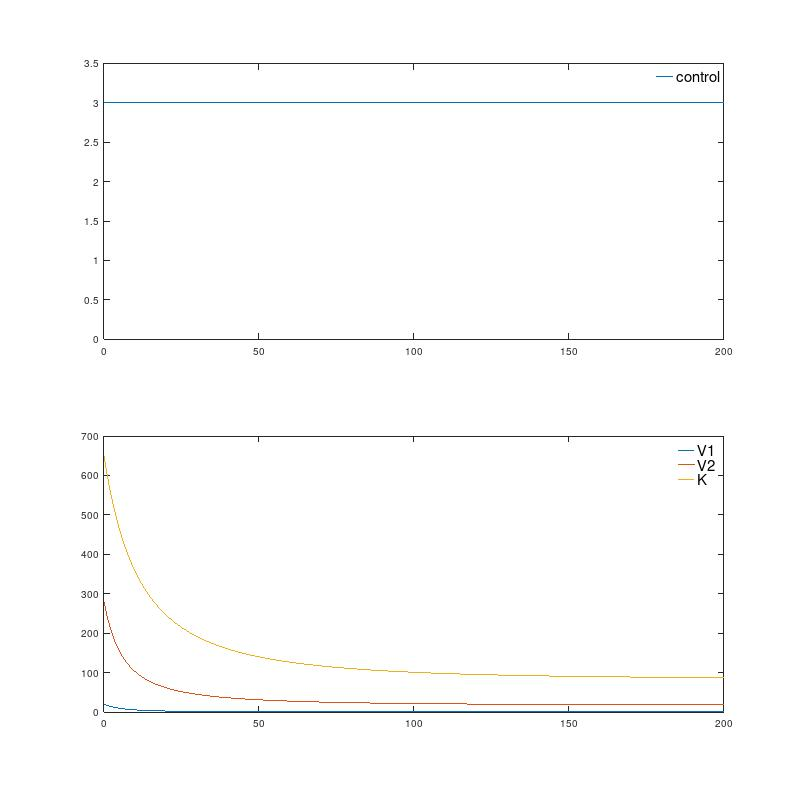
\includegraphics[width=.5\textwidth]{../plots/plot_max}
  \caption{Najlepsze znalezione rozwiązanie dla parametrów (CC)}\label{max_plot}
\end{figure}

Wyniki dla parametrów (CC)\ są dość jednoznaczne. Najmniejszą wartość $\hat{J}$ osiągamy dla sterowania $g \equiv g_{\max} = 3$, które zaprezentowano na Rysunku~\ref{max_plot}. Wszystkie testy zaczynające z tego sterowania zatrzymały się po jednej iteracji, patrz Tabela~\ref{param1_tbl}. Na podstawie tego, że norma lagrangianu w $g_3$ jest zerowa, możemy wnioskować, że rozwiązanie to jest minimum lokalnym naszego problemu.

Wyniki testów z Tabeli~\ref{param1_tbl} korzystające z siatki niejednorodnej wypadają zauważalnie gorzej od pozostałych. Widzimy też, że zmniejszenie Tol poprawiło wartość $\hat{J}$ w bardzo małym stopniu, a znacząco zwiększyło liczbę iteracji. Algorytm {\it sqp\/} jest jedynym który zbiegł z zerowego sterowania do sterowania optymalnego, co pokazuje że algorytm ten lepiej sprawuje się w powyższych przypadkach testowych.

Jako, że najlepsze znalezione, dla parametrów (CC), rozwiązanie trywializuje się, w dalszych eksperymentach skupimy się na parametrach~(DC), które dodatkowo zdają się prowadzić do nieciągłego optymalnego sterowania.

\subsection{Wpływ sterowania startowego}

\begin{table}[h]
  \begin{center}
    \begin{tabular}{|c|c|c|c|c|c|c||c|c|c|c|c|}
      \hline
      Param. & algorytm & aproks. & siatka & $h$ & start & Tol & $\hat{J}$ & iter & $\#\hat{J}$ & $\norm{L}_1$ & $\frac{\norm{L}_1}{\norm{L_0}_1}$ \\
      \hline
      (DC) & {\it lm\/} & $P_0$ & $S_{0.5}$ & 0.1 & $g_0$ & $10^{-6}$ & 3.04 & 81 & 158 & 141.46 & 47.286 \\
      \hline
      (DC) & {\it lm\/} & $P_0$ & $S_{0.5}$ & 0.1 & $g_0$ & $10^{-9}$ & 2.92 & 1003 & 1791 & 0.01 & 2.2e-03 \\
      \hline
      (DC) & {\it sqp\/} & $P_0$ & $S_{0.5}$ & 0.1 & $g_0$ & $10^{-6}$ & 3.3 & 18 & 205 & 21.37 & 7.145 \\
      \hline
      (DC) & {\it sqp\/} & $P_0$ & $S_{0.5}$ & 0.1 & $g_0$ & $10^{-9}$ & 3.3 & 18 & 205 & 21.37 & 7.145 \\
      \hline
      (DC) & {\it lm\/} & $P_0$ & $S_{0.5}$ & 0.1 & $g_3$ & $10^{-6}$ & 4.07 & 1 & 2 & 0.0 & --- \\
      \hline
      (DC) & {\it lm\/} & $P_0$ & $S_{0.5}$ & 0.1 & $g_3$ & $10^{-9}$ & 4.07 & 1 & 2 & 0.0 & --- \\
      \hline
      (DC) & {\it sqp\/} & $P_0$ & $S_{0.5}$ & 0.1 & $g_3$ & $10^{-6}$ & 4.07 & 1 & 2 & 0.0 & --- \\
      \hline
      (DC) & {\it sqp\/} & $P_0$ & $S_{0.5}$ & 0.1 & $g_3$ & $10^{-9}$ & 4.07 & 1 & 2 & 0.0 & --- \\
      \hline
      (DC) & {\it lm\/} & $P_0$ & $S_{0.5}$ & 0.1 & $g_{0,0.55,42.5}$ & $10^{-6}$ & 2.72 & 31 & 64 & 50.43 & 25.094 \\
      \hline
      (DC) & {\it lm\/} & $P_0$ & $S_{0.5}$ & 0.1 & $g_{0,0.55,42.5}$ & $10^{-9}$ & 2.69 & 412 & 722 & 0.49 & 0.242 \\
      \hline
      (DC) & {\it sqp\/} & $P_0$ & $S_{0.5}$ & 0.1 & $g_{0,0.55,42.5}$ & $10^{-6}$ & 2.71 & 10 & 130 & 3.62 & 1.799 \\
      \hline
      (DC) & {\it sqp\/} & $P_0$ & $S_{0.5}$ & 0.1 & $g_{0,0.55,42.5}$ & $10^{-9}$ & 2.71 & 10 & 130 & 3.62 & 1.799 \\
      \hline
      (DC) & {\it lm\/} & $P_0$ & $S_{0.5}$ & 0.1 & $g_{0.07,0.59,48.2}$ & $10^{-6}$ & 2.72 & 45 & 91 & 2.18 & 0.725 \\
      \hline
      (DC) & {\it lm\/} & $P_0$ & $S_{0.5}$ & 0.1 & $g_{0.07,0.59,48.2}$ & $10^{-9}$ & 2.69 & 811 & 1439 & 0.0 & 6.7e-04 \\
      \hline
      (DC) & {\it sqp\/} & $P_0$ & $S_{0.5}$ & 0.1 & $g_{0.07,0.59,48.2}$ & $10^{-6}$ & 2.76 & 5 & 93 & 6.16 & 2.045 \\
      \hline
      (DC) & {\it sqp\/} & $P_0$ & $S_{0.5}$ & 0.1 & $g_{0.07,0.59,48.2}$ & $10^{-9}$ & 2.76 & 5 & 93 & 6.16 & 2.045 \\
      \hline
    \end{tabular}
    \caption{Wpływ doboru sterowania startowego na przebieg optymalizacji}\label{start_tbl}
  \end{center}
\end{table}

Wyniki badające różne sterowania startowe dla różnych algorytmów i wartości tolerancji przedstawione zostały na Tabeli~\ref{start_tbl}. Pozwalają one na wyciągnięcie kilku ciekawych wniosków. Po pierwsze widzimy, że dla $\text{Tol} = 10^{-6}$ względne normy lagrangianów są bardzo duże, w szczególności prawie zawsze większe od 1. Oznacza to, że rozwiązania te są zapewne dalekie od optimów lokalnych, więc ta wartość Tol jest zapewne zbyt duża i dalej będziemy skupiać się na badaniu niższych wartości tolerancji. Ponadto wygląda na to, że zmniejszenie Tol nie poprawiło wyników algorytmu {\it sqp}.

Na Tabeli~\ref{start_tbl} widzimy, że norma lagrangianu dla rozwiązania $g_3$ wynosi 0, więc możemy wnioskować, że przy parametrach (DC), podobnie jak przy parametrach (CC), sterowanie $g_3$ (czyli stale równe $3 = g_{\max}$) jest minimum lokalnym. Jednak w tym przypadku wartości $\hat{J}$ są znacznie gorsze od pozostałych rezultatów. 

Najlepsze wartości $\hat{J}$ osiągane są przy sterowaniach startowych $g_{0,0.55,42.5}$ i $g_{0.07,0.59,48.2}$. Widzimy, że nawet dla Tol $= 10^{-6}$ wychodzą dobre wartości funkcjonału celu, ale dopiero ustawienie Tol na $10^{-9}$ pozwala uzyskać niskie wartości $\frac{\norm{L}_1}{\norm{L_0}_1}$ i tutaj wyraźnie lepiej wypada sterowanie startowe $g_{0.07,0.59,48.2}$. Warto też zauważyć, że pomimo podobnych wartości funkcji $\hat{J}$ dla tych czterech przypadków testowych, wynikowe sterowania zauważalnie się dla nich różnią, co pokazano na Rysunkach~\ref{test_g55_sol} i~\ref{test_gcomp_sol}.

Widzimy też, że dla startu $g_0$ przy Tol $= 10^{-9}$ i algorytmie {\it lm\/} udało się osiągnąć niską normę lagrangianu, jednak wartość $\hat{J}$ dla tego przypadku jest znacznie gorsza niż dla wcześniej wspomnianych przypadków. Wnioskujemy więc z tego, że dla tego punktu startowego optymalizator zbiega do nieoptymalnego minimum lokalnego. Potwierdzają to wyraźne różnice między kształtem sterowania uzyskanego dla tego przypadku, a wyżej omawianymi wynikami, które możemy zaobserwować porównując wykresy przedstawione na Rysunkach~\ref{test_zero_9},~\ref{p_55_9} i~\ref{p_comp_9}. Z tego powodu nie będziemy dalej zajmować się tym sterowaniem startowym.

\begin{figure}[h!]
  \begin{subfigure}{.5\textwidth}
    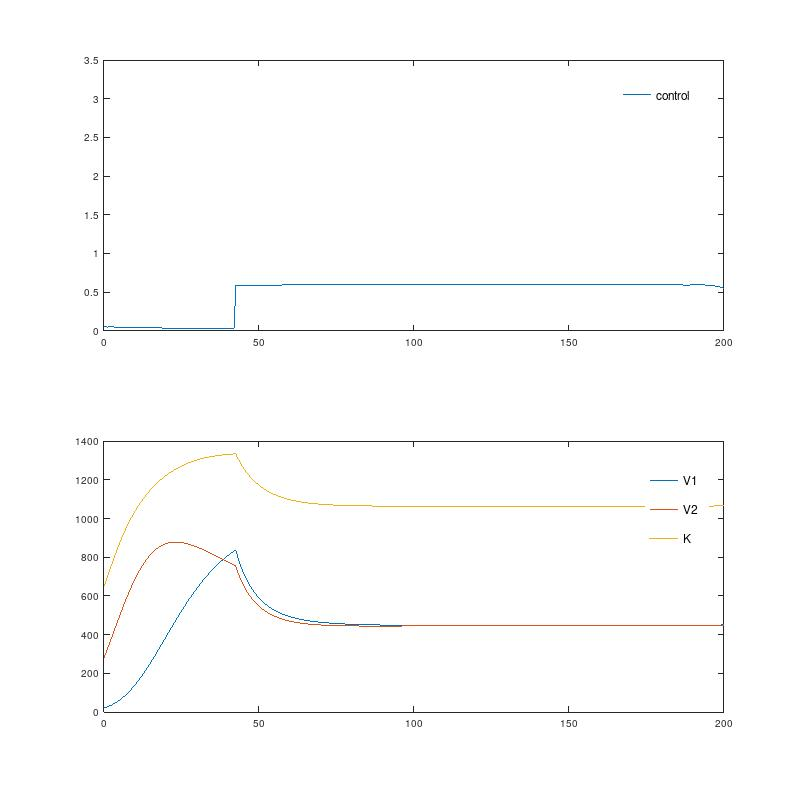
\includegraphics[width=\textwidth]{../plots/p_55_6}
    \caption{Tol = $10^{-6}$}\label{p_55_6}
  \end{subfigure}
  \begin{subfigure}{.5\textwidth}
    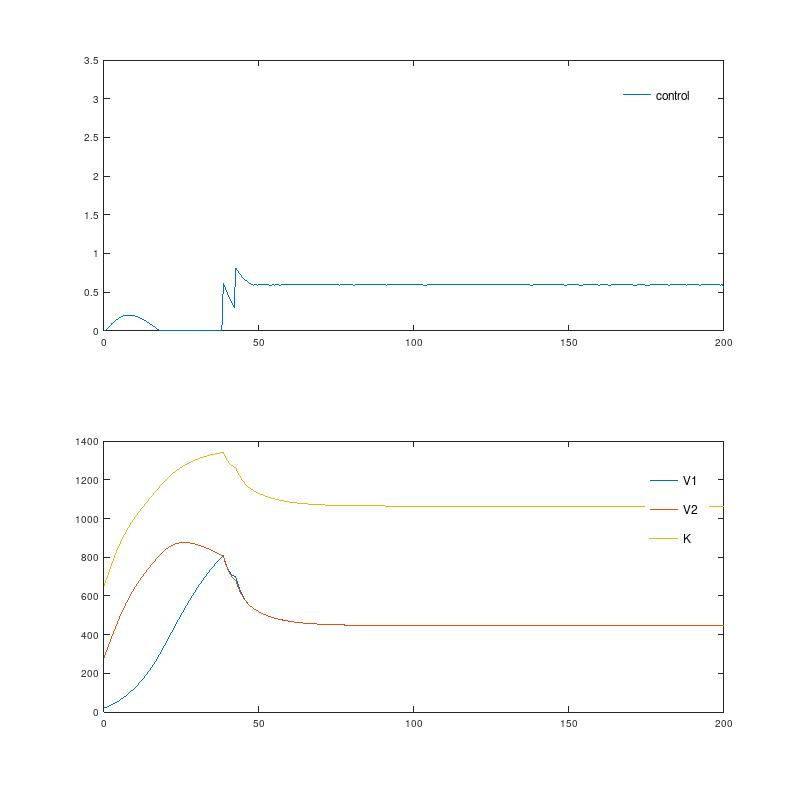
\includegraphics[width=\textwidth]{../plots/p_55_9}
    \caption{Tol = $10^{-9}$}\label{p_55_9}
  \end{subfigure}%
  \caption{Rozwiązania uzyskane przy użyciu sterowania startowego $g_{0,0.55,42.5}$}\label{test_g55_sol}
\end{figure}

\begin{figure}[h]
  \begin{subfigure}{.5\textwidth}
    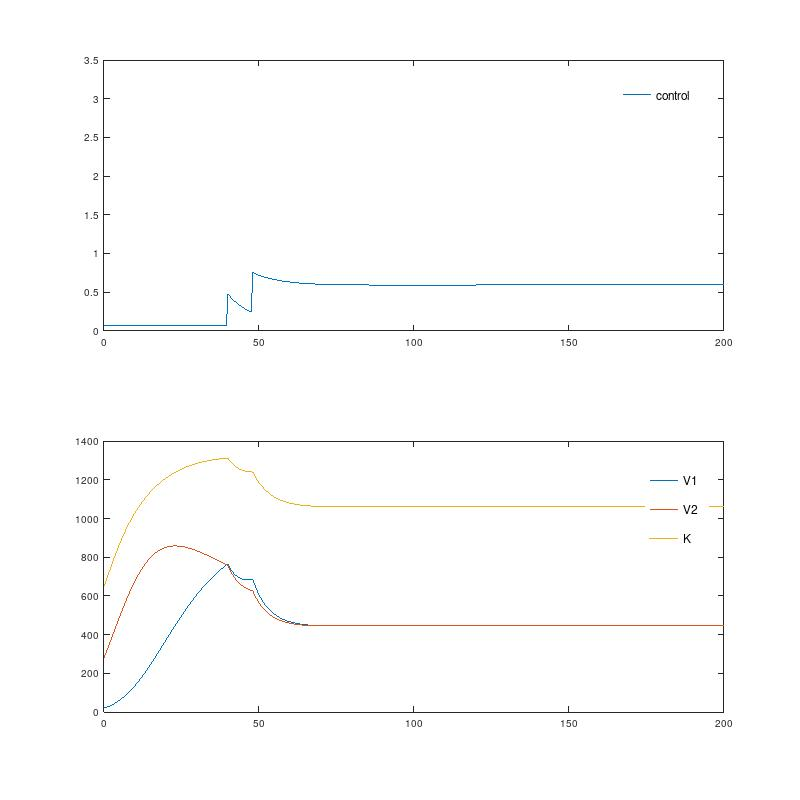
\includegraphics[width=\textwidth]{../plots/p_comp_6}
    \caption{Tol = $10^{-6}$}\label{p_comp_6}
  \end{subfigure}
  \begin{subfigure}{.5\textwidth}
    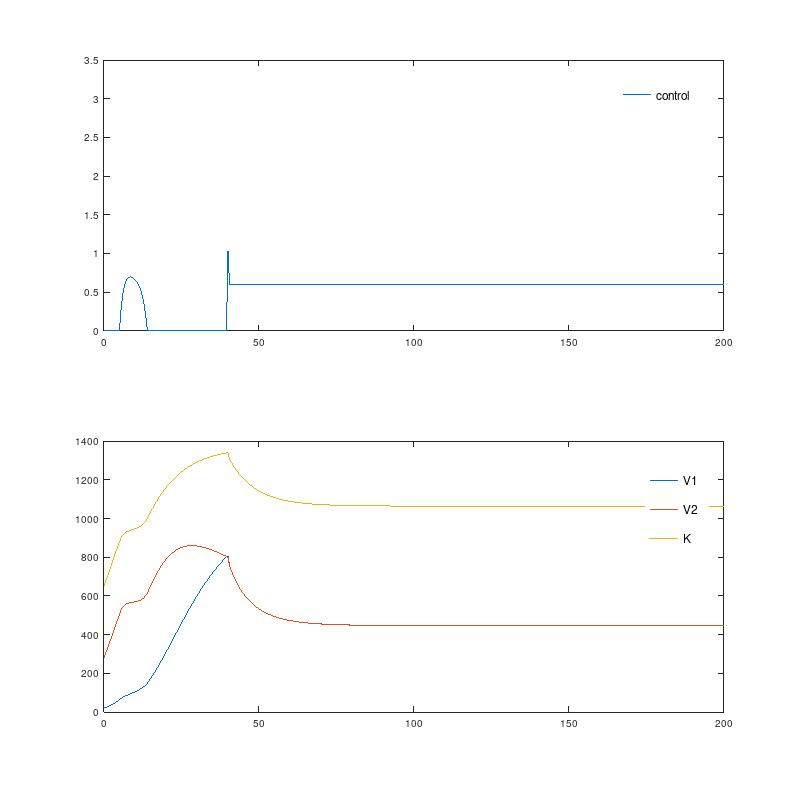
\includegraphics[width=\textwidth]{../plots/p_comp_9}
    \caption{Tol = $10^{-9}$}\label{p_comp_9}
  \end{subfigure}% 
  \caption{Rozwiązania uzyskane przy użyciu sterowania startowego $g_{0.07,0.59,48.2}$}\label{test_gcomp_sol}
\end{figure}

\begin{figure}[h]
  \centering
  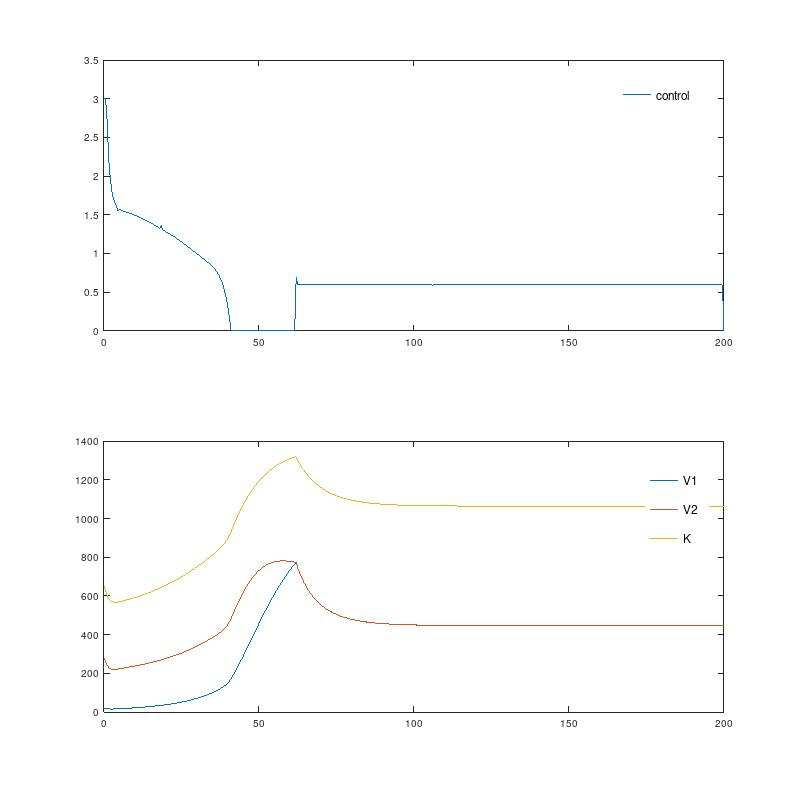
\includegraphics[width=.5\textwidth]{../plots/plot_zprc}
  \caption{Rozwiązanie uzyskane przy użyciu sterowania startowego $g_0$ i Tol $= 10^{-9}$}\label{test_zero_9}
\end{figure}

\subsection{Metoda dyskretyzacji}

\begin{table}[h!]
  \begin{center}
    \begin{tabular}{|c|c|c|c|c|c|c||c|c|c|c|c|}
      \hline
      Param. & algorytm & aproks. & siatka & $h$ & start & Tol & $\hat{J}$ & iter & $\#\hat{J}$ & $\norm{L}_1$ & $\frac{\norm{L}_1}{\norm{L_0}_1}$ \\
      \hline
      (DC) & {\it lm\/} & $P_0$ & $S_{0.5}$ & 0.1 & $g_{0.07,0.59,48.2}$ & $10^{-9}$ & 2.69 & 811 & 1439 & 0.0 & 6.7e-04 \\
      \hline
      (DC) & {\it lm\/} & $P_1$ & $S_{0.5}$ & 0.1 & $g_{0.07,0.59,48.2}$ & $10^{-9}$ & 2.76 & 1 & 6 & 4.54 & 1.0 \\
      \hline
      (DC) & {\it sqp\/} & $P_0$ & $S_{0.5}$ & 0.1 & $g_{0.07,0.59,48.2}$ & $10^{-9}$ & 2.76 & 5 & 93 & 6.16 & 2.045 \\
      \hline
      (DC) & {\it sqp\/} & $P_1$ & $S_{0.5}$ & 0.1 & $g_{0.07,0.59,48.2}$ & $10^{-9}$ & 2.76 & 5 & 101 & 7.06 & 1.556 \\
      \hline
    \end{tabular}
    \caption{Wpływ metody dyskretyzacji sterowania na przebieg optymalizacji}\label{discr_tbl}
  \end{center}
\end{table}

Jak widzimy na Tabeli~\ref{discr_tbl} dyskretyzacja kawałkami stała wydaje się osiągać znacznie lepsze rezultaty od optymalizacji kawałkami liniowej. Co prawda dla algorytmu {\it sqp\/} wynik wydaje się taki sam, a norma względna gradientu nawet lepsza, jednakże norma bezwzględna jest w tym przypadku zauważalnie gorsza. Problemy z dyskretyzacją $P_1$ są zapewne powodowane możliwą nieciągłością sterowania optymalnego i przybliżaniem nieciągłego sterowania $g_{0.07,0.59,48.2}$ sterowaniem kawałkami liniowym. Zakończenie optymalizacji po pierwszej iteracji przez algorytm {\it lm\/} jest spowodowane brakiem znalezienia lepszego sterowania w otoczeniu sterowania startowego, co z kolei może być powodowane błędami wynikającymi z przybliżania sterowania nieciągłego sterowaniem kawałkami liniowym.

\subsection{Siatka dyskretyzacji}

\begin{table}[h!]
  \begin{center}
    \begin{tabular}{|c|c|c|c|c|c|c||c|c|c|c|c|}
      \hline
      Param. & algorytm & aproks. & siatka & $h$ & start & Tol & $\hat{J}$ & iter & $\#\hat{J}$ & $\norm{L}_1$ & $\frac{\norm{L}_1}{\norm{L_0}_1}$ \\
      \hline
      (DC) & {\it lm\/} & $P_0$ & $S_1$ & 0.1 & $g_{0.07,0.59,48.2}$ & $10^{-9}$ & 2.7 & 620 & 1110 & 0.18 & 0.058 \\
      \hline
      (DC) & {\it lm\/} & $P_0$ & $S_{0.5}$ & 0.1 & $g_{0.07,0.59,48.2}$ & $10^{-9}$ & 2.69 & 811 & 1439 & 0.0 & 6.7e-04 \\
      
      \hline
      (DC) & {\it lm\/} & $P_0$ & $N_{sr}$ & 0.1 & $g_{0.07,0.59,48.2}$ & $10^{-9}$ & 2.7 & 280 & 505 & 2.86 & 1.237 \\
      \hline
      (DC) & {\it sqp\/} & $P_0$ & $S_1$ & 0.1 & $g_{0.07,0.59,48.2}$ & $10^{-9}$ & 2.76 & 11 & 187 & 5.45 & 1.812 \\
      \hline
      (DC) & {\it sqp\/} & $P_0$ & $S_{0.5}$ & 0.1 & $g_{0.07,0.59,48.2}$ & $10^{-9}$ & 2.76 & 5 & 93 & 6.16 & 2.045 \\
      \hline
      (DC) & {\it sqp\/} & $P_0$ & $N_{sr}$ & 0.1 & $g_{0.07,0.59,48.2}$ & $10^{-9}$ & 2.76 & 8 & 147 & 14.51 & 6.276 \\
      \hline
    \end{tabular}
    \caption{Wpływ doboru siatki dyskretyzacji na przebieg optymalizacji}\label{grid_tbl}
  \end{center}
\end{table}

Zgodnie z oczekiwaniami gęstsza siatka jednorodna osiąga lepsze wyniki dla algorytmu {\it lm}, co widzimy na Tabeli~\ref{grid_tbl}, natomiast siatka niejednorodna okazuje się osiągać gorsze wyniki od siatek jednorodnych. Co prawda wartości $\hat{J}$ dla siatki niejednorodnej są niewiele gorsze od tych dla siatki jednorodnej, a liczba iteracji znacznie mniejsza, ale po normach gradientu widzimy, że punkt do którego zbiegła optymalizacja jest znacznie odległy od minimum lokalnego. Dla algorytmu {\it sqp\/} wartości $\hat{J}$ są takie same dla każdej siatki, ale widzimy, że gradient wyniku jest najmniejszy dla siatki $S_1$, czyli w tym wypadku lepiej wypada rzadsza siatka jednorodna.

\subsection{Krok dyskretyzacji $h$}

\begin{table}[h]
  \begin{center}
    \begin{tabular}{|c|c|c|c|c|c|c||c|c|c|c|c|}
      \hline
      Param. & algorytm & aproks. & siatka & $h$ & start & Tol & $\hat{J}$ & iter & $\#\hat{J}$ & $\norm{L}_1$ & $\frac{\norm{L}_1}{\norm{L_0}_1}$ \\
      \hline
      (DC) & {\it lm\/} & $P_0$ & $S_{0.5}$ & 0.5 & $g_{0.07,0.59,48.2}$ & $10^{-9}$ & 2.69 & 974 & 1741 & 0.0 & 6.7e-04 \\
      \hline
      (DC) & {\it lm\/} & $P_0$ & $S_{0.5}$ & 0.1 & $g_{0.07,0.59,48.2}$ & $10^{-9}$ & 2.69 & 811 & 1439 & 0.0 & 6.7e-04 \\
      \hline
      (DC) & {\it lm\/} & $P_0$ & $S_{0.5}$ & 0.02 & $g_{0.07,0.59,48.2}$ & $10^{-9}$ & 2.76 & 1 & 6 & 2.95 & 1.0 \\
      \hline
      (DC) & {\it sqp\/} & $P_0$ & $S_{0.5}$ & 0.5 & $g_{0.07,0.59,48.2}$ & $10^{-9}$ & 2.76 & 3 & 66 & 9.55 & 2.824 \\
      \hline
      (DC) & {\it sqp\/} & $P_0$ & $S_{0.5}$ & 0.1 & $g_{0.07,0.59,48.2}$ & $10^{-9}$ & 2.76 & 5 & 93 & 6.16 & 2.045 \\
      \hline
      (DC) & {\it sqp\/} & $P_0$ & $S_{0.5}$ & 0.02 & $g_{0.07,0.59,48.2}$ & $10^{-9}$ & 2.76 & 5 & 100 & 17.14 & 5.814 \\
      \hline
    \end{tabular}
    \caption{Wpływ doboru kroku dyskretyzacji $h$ na przebieg optymalizacji}\label{step_tbl}
  \end{center}
\end{table}

Wyniki eksperymentów badających wpływ dobory kroku dyskretyzacji $h$ przestawiono na Tabeli~\ref{step_tbl}. Widzimy, że przy obniżeniu długości kroku z $0.5$ do $0.1$ wyniki się poprawiły. Dla algorytmu {\it lm\/} spadła liczba potrzebnych iteracji, a dla algorytmu {\it sqp\/} spadła norma lagrangianu. Przy dalszym obniżaniu kroku $h$ wyniki wydają się pogarszać, w szczególności dla algorytmu {\it lm}, któremu nie udało się znaleźć żadnego sterowania lepszego od sterowania startowego i zakończył optymalizację po pierwszej iteracji. Zauważmy tutaj, że dla różnych długości kroków $h$ rozpatrujemy faktycznie inne zadanie, więc takie zachowanie jest możliwe.

\subsection{Warunek stopu}

\begin{table}[h]
  \begin{center}
    \begin{tabular}{|c|c|c|c|c|c|c||c|c|c|c|c|}
      \hline
      Param. & algorytm & aproks. & siatka & $h$ & start & Tol & $\hat{J}$ & iter & $\#\hat{J}$ & $\norm{L}_1$ & $\frac{\norm{L}_1}{\norm{L_0}_1}$ \\
      \hline
      (DC) & {\it lm\/} & $P_0$ & $S_{0.5}$ & 0.1 & $g_{0.07,0.59,48.2}$ & $10^{-6}$ & 2.72 & 45 & 91 & 2.18 & 0.725 \\
      \hline
      (DC) & {\it lm\/} & $P_0$ & $S_{0.5}$ & 0.1 & $g_{0.07,0.59,48.2}$ & $10^{-9}$ & 2.69 & 811 & 1439 & 0.0 & 6.7e-04 \\
      \hline
      (DC) & {\it lm\/} & $P_0$ & $S_{0.5}$ & 0.1 & $g_{0.07,0.59,48.2}$ & $10^{-11}$ & 2.69 & 1314 & 2313 & 0.0 & 3.7e-05 \\
      \hline
      (DC) & {\it lm\/} & $P_0$ & $S_{0.5}$ & 0.1 & $g_{0.07,0.59,48.2}$ & $10^{-13}$ & 2.69 & 1401 & 2466 & 0.0 & 5.7e-04 \\
      \hline
      (DC) & {\it sqp\/} & $P_0$ & $S_{0.5}$ & 0.1 & $g_{0.07,0.59,48.2}$ & $10^{-6}$ & 2.76 & 5 & 93 & 6.16 & 2.045 \\
      \hline
      (DC) & {\it sqp\/} & $P_0$ & $S_{0.5}$ & 0.1 & $g_{0.07,0.59,48.2}$ & $10^{-9}$ & 2.76 & 5 & 93 & 6.16 & 2.045 \\
      \hline
      (DC) & {\it sqp\/} & $P_0$ & $S_{0.5}$ & 0.1 & $g_{0.07,0.59,48.2}$ & $10^{-11}$ & 2.76 & 5 & 93 & 6.16 & 2.045 \\
      \hline
      (DC) & {\it sqp\/} & $P_0$ & $S_{0.5}$ & 0.1 & $g_{0.07,0.59,48.2}$ & $10^{-13}$ & 2.76 & 5 & 93 & 6.16 & 2.045 \\
      \hline
    \end{tabular}
    \caption{Wpływ warunku stopu na przebieg optymalizacji}\label{tol_tbl}
  \end{center}
\end{table}

Najlepsze wyniki na Tabeli~\ref{tol_tbl} osiągane są dla Tol $= 10^{-11}$. Przy Tol $= 10^{-6}$ norma $\norm{G}_1$ jest duża, więc rozwiązanie uzyskane w ten sposób jest raczej odległe od minimum lokalnego. Widzimy też poprawę normy względnej lagrangianu o rząd wielkości przy obniżeniu wartości Tol z $10^{-9}$ do $10^{-11}$, choć należy zauważyć, że poprawa ta wymagała przeprowadzenia aż 500 dodatkowych iteracji. Przy dalszym obniżaniu Tol do $10^{-13}$ wyniki wydają się pogarszać, więc zapewne optymalna wartość Tol dla tego przypadku jest bliska $10^{-11}$.

Ten eksperyment potwierdza nasze podejrzenia, że dla algorytmu {\it sqp\/} parametr tolerancji nie ma wpływu na wynik w naszych eksperymentach, a wyniki osiągane przez ten algorytm wydają się być dalekie od minimum zarówno lokalnego jak i globalnego.

Podsumowując najlepsze wyniki udało się osiągnąć przy użyciu algorytmu {\it lm}, aproksymacji kawałkami stałej, siatki $S_{0.5}$ i kroku $h = 0.1$, zaczynając ze sterowania $g_{0.07,0.59,48.2}$, przy wartości parametru tolerancji $10^{-11}$. Są one zaprezentowane na Rysunku~\ref{plot_best_dc}.

\begin{figure}[h]
  \centering
  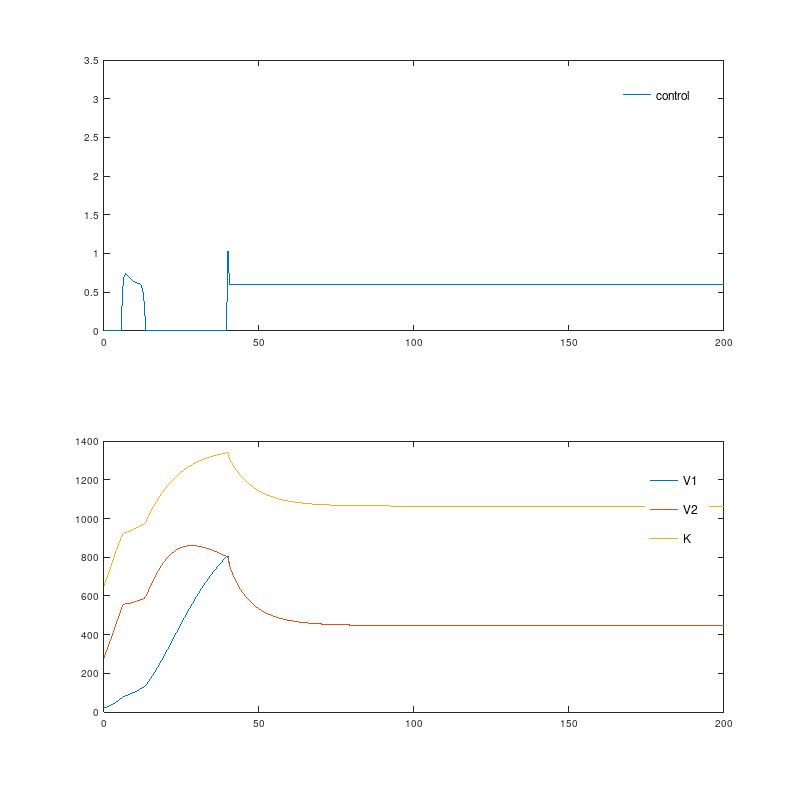
\includegraphics[width=.5\textwidth]{../plots/plot_best_dc}
  \caption{Najlepsze znalezione rozwiązanie dla parametrów (DC)}\label{plot_best_dc}
\end{figure}

\section{Dyskusja wyników}

Jak widzimy, wyniki dla parametrów (CC) i (DC) znacznie się różnią. Dokładniejsze przyjrzenie się funkcjonałowi celu (\ref{objfsim}) pozwala uzasadnić takie zjawisko na poziomie intuicji. Jak widzimy parametr $\omega$ jest mnożony przez wartość drugiej całki. Zauważmy, że funkcja pod drugą całką jest gładkim przybliżeniem funkcji znaku wyrażenia $y_2(t) - y_1(t)$. W przypadku (DC) parametr $\omega$ jest znacznie większy niż w (CC), więc w tym przypadku druga całka ma większy wpływ na wynik funkcjonału. Jak przyjrzymy się rozwiązaniu z np. Rysunku~\ref{p_comp_9}, widzimy, że punkt nieciągłości znajduje się od razu po przecięciu się krzywych $y_1$ i $y_2$, a po nim sterowanie ma taką wartość aby krzywe te były bardzo blisko siebie, ale przy zachowaniu $y_2(t) - y_1(t) < 0$. Wygląda więc na to, przy parametrach (DC)\ bardziej opłaca się utrzymywać stan $y_2(t) - y_1(t) < 0$, natomiast przy parametrach (CC)\ lepsze wyniki daje minimalizacja pierwszej całki, czyli pola pod $y_1 + y_2$. Możemy się też spodziewać, że wysokie wartości sterowania powodują zmniejszanie się zarówno $y_1$ jak i $y_2$, ale od pewnej wartości sterowania $y_1$ maleje szybciej niż $y_2$. Taka hipoteza zgadzałaby się z interpretacją $y_1$ i $y_2$ jako liczba komórek nowotworowych odpowiednio podatnych na działanie leku i odpornych na niego, a wartości sterowania jako dawki leku.

Otrzymywane normy względne lagrangianów były dość niewielkie dla najlepszych otrzymywanych wyników. Sugeruje to, że otrzymywane wyniki są bliskie optimom lokalnym. Należy jednak pamiętać, że nie jest to jeszcze dowód i wyniki te mogą jednak okazać się odległe od optimów lokalnych. Ponadto otrzymywane wyniki były mocno zależne od punktu startowego, co pozwala podejrzewać, że istnieją punkty startowe dla których moglibyśmy osiągnąć znacznie lepsze wyniki. W szczególności podejrzewamy, że sterowania startowe z różnymi punktami nieciągłości prowadzą do innych optimów lokalnych. Podejrzenia te są oparte na obserwacji, że optymalizacja, zaczynając z nieciągłego sterowania, kończyła się zwykle wynikiem mającym nieciągłość w tym samym punkcie. Być może zastosowanie innych algorytmów optymalizacji nieliniowej umożliwiłoby szukanie rozwiązania w sposób mniej zależący od znalezienia dobrego punktu startowego. Może też da się sformalizować heurystyczną metodę poszukiwania punktu startowego opisaną w rozdziale~\ref{start_method}, oraz uzyskać za jej pomocą znacznie lepsze wyniki. Ostatecznie, być może przyjęta przez nas metoda ,,direct single shooting'' nie jest dobrym wyborem dla tego zadania. Być może użycie np. metody ,,direct collocation'' pozwoliłoby osiągnąć lepsze,\ bliższe lokalnemu i globalnemu minimum wyniki.

Niejednorodna siatka dyskretyzacji jest metodą nierzadko pozwalającą na poprawę tempa zbieżności, ale nie udało się jej tu z sukcesem zastosować. Podobnie przybliżanie sterowania za pomocą splajnu wyższego rzędu też mogłoby poprawić tempo zbieżności. W literaturze rozważa się też metody automatyzacji znajdowania siatki dyskretyzacji i odpowiedniego rzędu dyskretyzacji. Przykładem jest tu praca~\cite{Rao-ph}. Być może zastosowanie ich umożliwiłoby uzyskanie lepszych wyników.

Dla parametrów (DC) nie udało nam się skutecznie zastosować algorytmu {\it sqp}. Algorytm ten potrafi osiągać dobre wyniki, co mogliśmy zaobserwować w przypadku (CC), dla którego osiągnął on znacznie lepsze rezultaty niż {\it lm\_feasible}. Podejrzewamy, że problemem w naszym przypadku były zbyt luźne warunki zakończenia optymalizacji tego algorytmu.  Niestety dokumentacja algorytmu {\it sqp\/}  nie specyfikuje jakie są warunki zakończenia optymalizacji i na co wpływa parametr ,,octave\_sqp\_tolerance''. Ponadto, zgodnie z dokumentacją, jest to jedyny parametr służący do kontrolowania warunków zakończenia optymalizacji używany przez ten algorytm.

Przypomnijmy jeszcze uwagę z początku pracy, że gdy $y_1 = y_2 = 0$, lub $y_3 = 0$ to zadanie nie jest dobrze określone, a w przypadku gdy wartości te są bliskie zeru, mogą występować znaczne błędy numeryczne. W żadnym eksperymencie wartości $y_1$ ani $y_2$ nie były bliskie zeru. Minimalna wartość $y_3$ z Rysunku~\ref{max_plot} to $14.9$, więc i ta nie jest zbyt bliska 0. Okazuje się jednak, że przy parametrach (DC), w rozwiązaniu (\ref{odesim}) dla sterowania stale równego $g_{\max}$ minimalna wartość $y_3$ wynosi ok. $0.02$. Nie jest to wartość na tyle mała, by móc powodować istotne błędy, ale jej występowanie sygnalizuje, że w innych eksperymentach być może pojawiają się mniejsze wartości.

Zauważmy, że najlepsze otrzymywane wyniki dla parametrów (DC) sugerują, że optymalne sterowanie jest nieciągłe. Jeśli jest tak w rzeczywistości, to zapewne wszystkie nasze przybliżenia obarczone są pierwotnym błędem aproksymacji, powodowanym faktem, że prawie na pewno optymalny punkt nieciągłości nie należy do naszej siatki dyskretyzacji. Zauważmy też, że użyte przez nas metody, w szczególności aproksymacja sterowania przez funkcję kawałkami stałą, oraz dostosowanie długości kroku $h$ algorytmu R-K do długości przedziału dyskretyzacji, mogą skutecznie ograniczać skutki możliwej nieciągłości optymalnego sterowania. Wskazywać na to mogą na przykład zauważalnie lepsze wyniki dyskretyzacji kawałkami stałej w porównaniu do dyskretyzacji kawałkami liniowej, które możemy zaobserwować na Tabeli~\ref{discr_tbl}.

Na koniec należy podkreślić znaczenie zaimplementowania funkcji obliczającej gradient $\hat{J}$. Pozwoliło to znacząco zmniejszyć liczbę obliczeń funkcjonału celu $\hat{J}$. Asymptotyczna liczba obliczeń $\hat{J}$ wykonywanych w jednej iteracji optymalizacji spadła z liniowej wzgl.\ liczby parametrów do stałej. Przykładowo w eksperymentach zawierających 400 parametrów i wymagających 1000 iteracji, pozwoliło no przyspieszyć obliczenia ok. 100 razy.

\chapter{Podsumowanie}
W tej pracy sprowadziliśmy problem optymalnej strategii podawania leku do problemu optymalizacji nieliniowej z ograniczeniami, korzystając z metody ,,direct single shooting''. Jedną z istotnych cech podejścia było opracowanie procedury obliczającej (dokładny) gradient funkcji celu, z pominięciem aproksymacji różnicami skończonymi, która jest kosztowna obliczeniowo i może skutkować istotnymi błędami przybliżenia. Przeprowadziliśmy też testy potwierdzające poprawność naszej implementacji, przez porównanie z różnicową aproksymacją gradientu.

Przeprowadzone eksperymenty pozwoliły ustalić, że w przypadku tego zadania potencjalnie lepsze wyniki udaje się osiągać przy użyciu algorytmu {\it lm\_feasible\/} niż {\it sqp\/} oraz przybliżaniu sterowania funkcją kawałkami stałą niż kawałkami liniową. Oszacowaliśmy też optymalną, dla tego problemu, długość kroku dyskretyzacji algorytmu R-K na $0.1$, oraz wartość parametru tolerancji optymalizatora na $10^{-11}$. Omówiliśmy ponadto możliwe zagrożenia dla naszego rozwiązania, takie jak potencjalna nieciągłość optymalnego sterowania, brak zbieżności globalnej, czy możliwa znaczna odległość wyniku optymalizacji od minimum lokalnego.

Po przeanalizowaniu otrzymanych wyników, dochodzimy do wniosku, że wyglądają one obiecująco, ale nie nadają się jeszcze do wykorzystania w praktyce. Zastosowana metoda wydaje się mieć potencjał, ale dalsza praca jest potrzebna aby zweryfikować jakość i optymalność uzyskanych wyników. Niewątpliwie warto też sprawdzić alternatywne podejścia, jak np. metodę ,,direct collocation''. Mogą one umożliwić uzyskanie lepszych wyników, oraz dać pewien punkt odniesienia co do jakości uzyskanych przez nas wyników.

\newpage{}
\bibliography{bibliography}{}
\bibliographystyle{abbrv}
\end{document}
